\section{Moving Average Model}
\label{sec:MA}
A Moving Average (MA) model is another approach used in univariate time series analysis. Unlike the Autoregressive (AR) model, where the target variable depends on its past values, the MA model relies on past errors. \\
Formally, a Moving Average model of order $q$ is represented as:
\begin{equation}
    \label{eq:MA}
    y_{t} = \mu_{0} + \sum^{q}_{i=1} \theta_{i} \epsilon_{t-i} + \epsilon_t
\end{equation}
where $q$ is the number of past errors considered, $\mu_{0}$ is the mean of the series, $\theta_{1}, \theta_{2}, ..., \theta_{q}$ are the model coefficients, and $\epsilon_{t}, \epsilon_{t-1}, ..., \epsilon_{t-q}$ are the error terms. \\
For our analysis, we implemented the MA model of order 1 (MA(1)) and order 2 (MA(2)).

\subsection*{MA(1)}
The MA(1) model is defined as follows:
\begin{equation}
    \label{eq:MA1}
    y_{t} = \mu_{0} + \theta \epsilon_{t-1} + \epsilon_t
\end{equation}
In our case study, we assume that $\epsilon_t$ are independent and identically distributed variables from a normal distribution with mean $0$ and variance $\sigma^2$, i.e., $\epsilon_t \stackrel{iid}{\sim} \mathcal{N}(0,\sigma^2)$, leading to the following likelihood:
\begin{equation}
    \label{eq:MA1_likelihood}
    y_{t}|\mu_{0},\theta,\sigma^2,\epsilon_{t-1} \sim \mathcal{N}(\mu_{0} + \theta \epsilon_{t-1}, \sigma^2)
\end{equation}
For the priors, we chose:
\begin{equation}
    \label{eq:MA1_priors}
    \begin{split}
        \mu_0 \sim \mathcal{N}(0.0, 10000) \\
        \tau = 1 / \sigma^2 \sim \mathcal{G}(2, 0.1) \\
        \theta \sim \mathcal{U}(-1.0, 1.0)
    \end{split}
\end{equation}
We selected uninformative priors for all the parameters: $\mu_{0}$, $\sigma^2$, and $\theta$. \\
Running the JAGS code to implement the MA(1) model for GDP and CPIAUCSL, we obtained the posterior distributions shown in Figure \ref{fig:MA1_posteriors}, with the corresponding means and 95\% credible intervals reported in Table \ref{tab:MA1_posteriors}. \\
\begin{figure}[h]
    \centering
    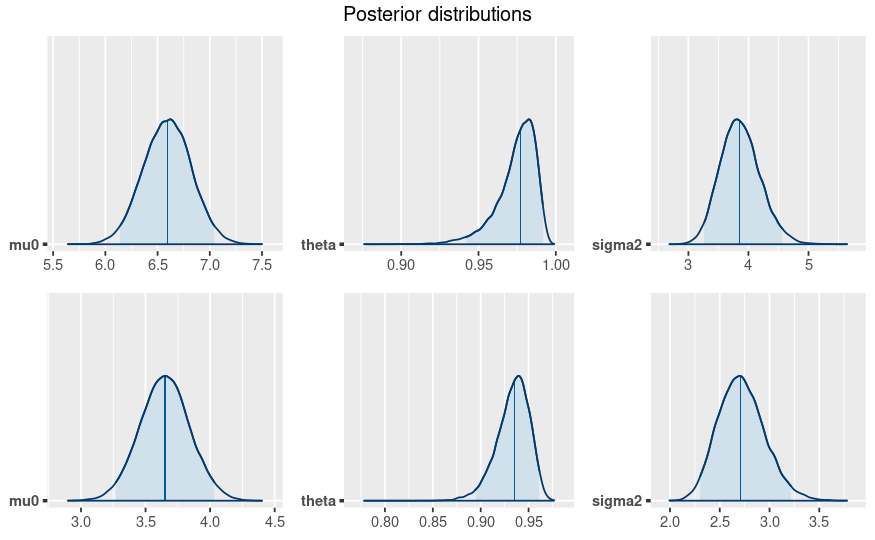
\includegraphics[width=0.8\textwidth]{images/3-MA/posteriors.png}
    \caption{Posterior distributions of the parameters for the MA(1) models. The top line corresponds to the model used for GDP, while the bottom line corresponds to the model used for CPIAUCSL.}
    \label{fig:MA1_posteriors}
\end{figure}
\begin{table}[H]
    \centering
    \begin{tabular}{|c|c|c|c|}
        \hline
        \textbf{Model target variable } & \textbf{Parameter } & \textbf{Posterior Mean } & \textbf{95\% Credible Interval } \\
        \hline
        GDP      & $\mu_0$    & 6.5934423 & (6.1441382, 7.0421211) \\
        GDP      & $\theta$   & 0.9745347 & (0.9419309, 0.9915436) \\
        GDP      & $\sigma^2$ & 3.8669139 & (3.2666059, 4.5663869) \\
        CPIAUCSL & $\mu_0$    & 3.6496595 & (3.2718468, 4.0311333) \\
        CPIAUCSL & $\theta$   & 0.9335022 & (0.8946139, 0.9613808) \\
        CPIAUCSL & $\sigma^2$ & 2.7205353 & (2.3038087, 3.2125894) \\
        \hline
    \end{tabular}
    \caption{Posterior means and 95\% credible intervals for the parameters of the MA(1) models.}
    \label{tab:MA1_posteriors}
\end{table}
In both the GDP and CPIAUCSL models, the $\theta$ parameter is close to 1. However, using a prior for $\theta$ over a larger range, i.e., $\theta \sim \mathcal{U}(-2.0, 2.0)$, did not significantly change the estimated value of $\theta$. \\
We also examined the trace plots and autocorrelation plots and found no significant issues. \\
Finally, plotting the in-sample and out-of-sample predictions with 95\% credible intervals and comparing them with the actual data, we obtained the results shown in Figures \ref{fig:MA1_gdp_prediction} and \ref{fig:MA1_infl_prediction}. As observed, the MA(1) model is not good for out of sample predictions, as it fails to capture the trend of the data and returns a flat line.
\begin{figure}[H]
    \centering
    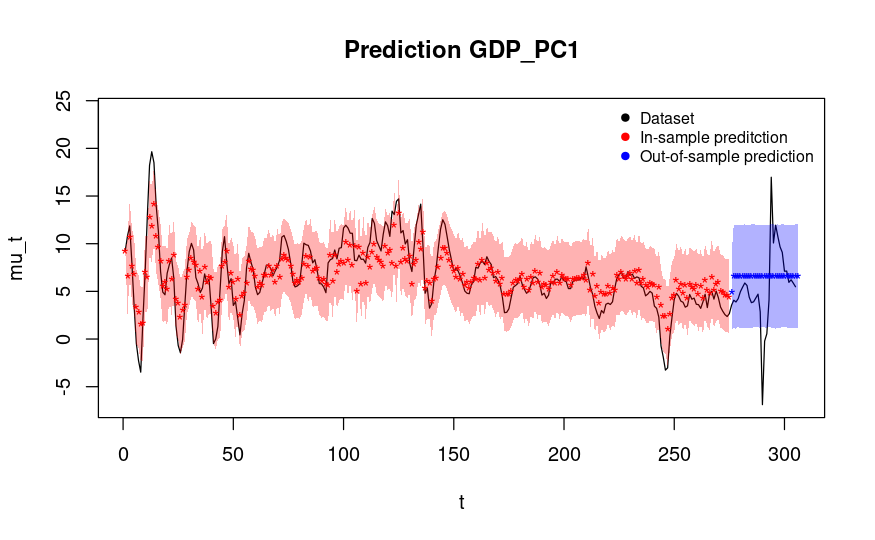
\includegraphics[width=0.75\textwidth]{images/3-MA/gdp_prediction.png}
    \caption{In-sample and out-of-sample predictions for the GDP using the MA(1) model.}
    \label{fig:MA1_gdp_prediction}
\end{figure}
\begin{figure}[H]
    \centering
    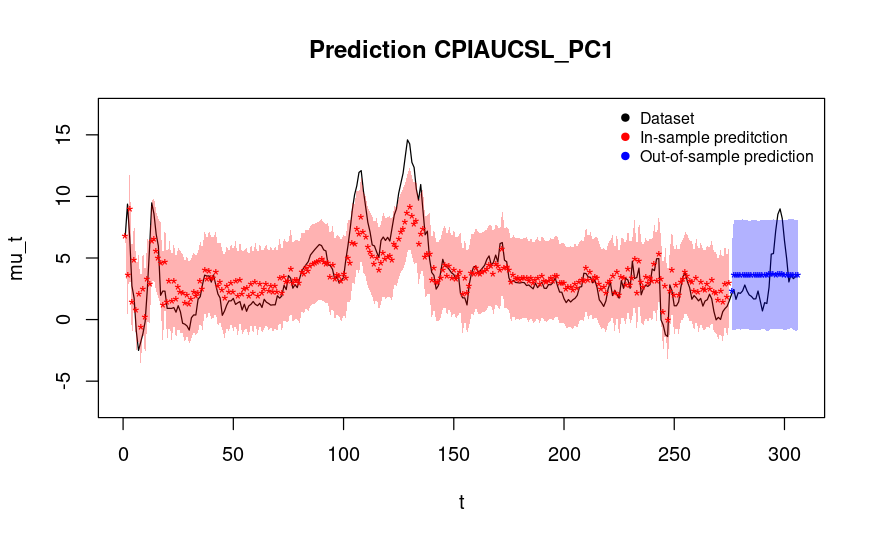
\includegraphics[width=0.75\textwidth]{images/3-MA/infl_prediction.png}
    \caption{In-sample and out-of-sample predictions for the CPIAUCSL using the MA(1) model.}
    \label{fig:MA1_infl_prediction}
\end{figure}
We also compared the model's in-sample predictions and posterior distributions with those obtained from the MA model using the ARIMA function. Detailed comparison results are provided in the Appendix, showing no significant differences between them.
\subsection*{MA(2)}
The MA(2) model is defined as follows:
\begin{equation}
    \label{eq:MA2}
    y_{t} = \mu_{0} + \theta_1 \epsilon_{t-1} + \theta_2 \epsilon_{t-2} + \epsilon_t
\end{equation}
In our case study, we assume that $\epsilon_t$ are independent and identically distributed variables from a normal distribution with mean $0$ and variance $\sigma^2$, i.e., $\epsilon_t \stackrel{iid}{\sim} \mathcal{N}(0,\sigma^2)$, leading to the following likelihood:
\begin{equation}
    \label{eq:MA2_likelihood}
    y_{t}|\mu_{0},\theta_1,\theta_2,\sigma^2,\epsilon_{t-1},\epsilon_{t-2} \sim \mathcal{N}(\mu_{0} + \theta_1 \epsilon_{t-1} + \theta_2 \epsilon_{t-2}, \sigma^2)
\end{equation}
For the priors, we chose:
\begin{equation}
    \label{eq:MA2_priors}
    \begin{split}
        \mu_0 \sim \mathcal{N}(0.0, 10000) \\
        \tau = 1 / \sigma^2 \sim \mathcal{G}(2, 0.1) \\
        \theta_1 \sim \mathcal{U}(-1.5, 1.5) \\
        \theta_2 \sim \mathcal{U}(-1.0, 1.0)
    \end{split}
\end{equation}
We selected uninformative priors for $\mu_{0}$, $\sigma^2$, $\theta_1$, and $\theta_2$. \\
Running the JAGS code to implement the MA(2) model for GDP and CPIAUCSL, we obtained the posterior distributions shown in Figure \ref{fig:MA2_posteriors}, with the corresponding means and 95\% credible intervals reported in Table \ref{tab:MA2_posteriors}. \\
\begin{figure}[H]
    \centering
    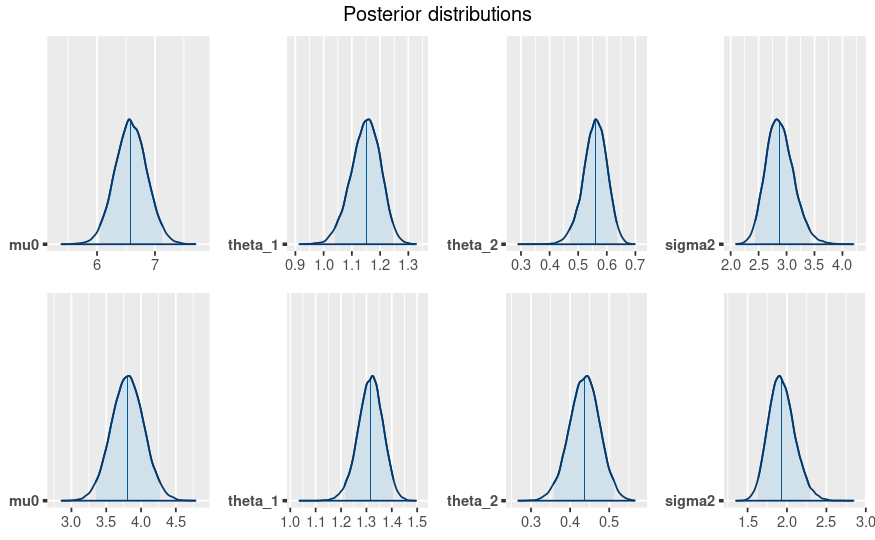
\includegraphics[width=0.8\textwidth]{images/3-MA/posteriors2.png}
    \caption{Posterior distributions of the parameters for the MA(2) models. The top line corresponds to the model used for GDP, while the bottom line corresponds to the model used for CPIAUCSL.}
    \label{fig:MA2_posteriors}
\end{figure} 
\begin{table}[H]
    \centering
    \begin{tabular}{|c|c|c|c|}
        \hline
        \textbf{Model target variable } & \textbf{Parameter } & \textbf{Posterior Mean } & \textbf{95\% Credible Interval } \\
        \hline
        GDP      & $\mu_0$    & 6.5862752 & (6.0523533, 7.1291252) \\
        GDP      & $\theta_1$ & 1.1489023 & (1.0408063, 1.2447200) \\
        GDP      & $\theta_2$ & 0.5587509 & (0.4698359, 0.6348533) \\
        GDP      & $\sigma^2$ & 2.8842617 & (2.4383601, 3.4118375) \\
        CPIAUCSL & $\mu_0$    & 3.8081535 & (3.3497252, 4.2727049) \\
        CPIAUCSL & $\theta_1$ & 1.3155230 & (1.2142974, 1.4063565) \\
        CPIAUCSL & $\theta_2$ & 0.4365283 & (0.3581476, 0.5111502) \\
        CPIAUCSL & $\sigma^2$ & 1.9356539 & (1.6371395, 2.2893457) \\
        \hline
    \end{tabular}
    \caption{Posterior means and 95\% credible intervals for the parameters of the MA(2) models.}
    \label{tab:MA2_posteriors}
\end{table}
Plotting the in-sample and out-of-sample predictions with 95\% credible intervals and comparing them with the actual data, we obtained the results shown in Figures \ref{fig:MA2_gdp_prediction} and \ref{fig:MA2_infl_prediction}. \\
As with the MA(1) model, the MA(2) model is not good for out-of-sample predictions, as it fails to capture the trend of the data and returns a flat line.
\begin{figure}[H]
    \centering
    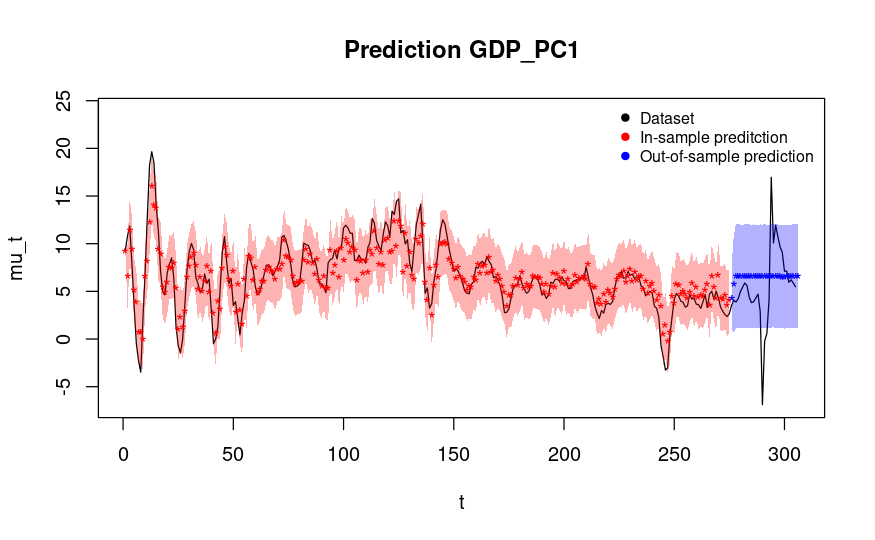
\includegraphics[width=0.75\textwidth]{images/3-MA/gdp_prediction2.png}
    \caption{In-sample and out-of-sample predictions for the GDP using the MA(2) model.}
    \label{fig:MA2_gdp_prediction}
\end{figure}
\begin{figure}[H]
    \centering
    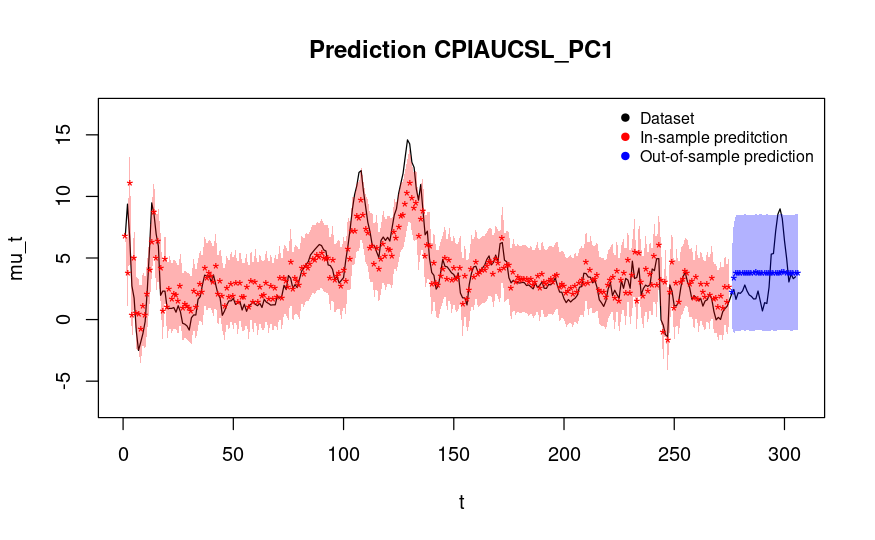
\includegraphics[width=0.75\textwidth]{images/3-MA/infl_prediction2.png}
    \caption{In-sample and out-of-sample predictions for the CPIAUCSL using the MA(2) model.}
    \label{fig:MA2_infl_prediction}
\end{figure}
In the end, we compared the model's in-sample predictions and posterior distributions with those obtained from the MA model using the ARIMA function. Detailed comparison results are provided in the Appendix, showing no significant differences between them.